\documentclass[11pt,a4paper]{article}

\usepackage[T1]{fontenc}
\usepackage[utf8]{inputenc}
\usepackage{lmodern}
\usepackage{amssymb}
\usepackage[margin=24mm]{geometry}
\usepackage{xcolor}
\usepackage{microtype}
\DisableLigatures{encoding=T1,family=tt*}
\usepackage{enumitem}
\usepackage{booktabs}
\usepackage{tabularx}
\usepackage{listings}
\usepackage{tikz}
\usetikzlibrary{arrows.meta,positioning}
\usepackage{fancyhdr}
\usepackage{hyperref}

\definecolor{ZipperInk}{HTML}{17212B}
\definecolor{ZipperBlue}{HTML}{176B87}
\definecolor{ZipperLight}{HTML}{EEF6F8}
\definecolor{CodeBackground}{HTML}{F5F7F8}
\definecolor{CodeComment}{HTML}{58715D}
\definecolor{WarningBorder}{HTML}{B7791F}

\hypersetup{
  colorlinks=true,
  linkcolor=ZipperBlue,
  urlcolor=ZipperBlue,
  pdftitle={Call Intake with ZipperGen Studio},
  pdfauthor={The ZipperGen Authors}
}

\pagestyle{fancy}
\fancyhf{}
\lhead{Call intake with ZipperGen Studio}
\rhead{End-to-end check}
\cfoot{\thepage}
\setlength{\headheight}{14pt}

\setlist[itemize]{topsep=4pt,itemsep=2pt}
\setlist[enumerate]{topsep=4pt,itemsep=3pt}
\setlength{\parindent}{0pt}
\setlength{\parskip}{6pt}

\lstset{
  basicstyle=\ttfamily\small,
  backgroundcolor=\color{CodeBackground},
  frame=single,
  rulecolor=\color{black!18},
  breaklines=true,
  breakatwhitespace=false,
  columns=fullflexible,
  keepspaces=true,
  showstringspaces=false,
  upquote=true,
  numbers=none
}

\lstdefinestyle{shell}{
  language=bash,
  numbers=none
}

\tikzset{
  zgstage/.style={
    draw=ZipperBlue,
    fill=ZipperLight,
    very thick,
    rounded corners=2.5pt,
    align=center,
    minimum height=12mm,
    inner sep=4pt,
    font=\small
  },
  zgflow/.style={-{Latex[length=2.2mm,width=1.5mm]}, thick, draw=ZipperBlue}
}

\newenvironment{notebox}[1]
{\begin{center}\begin{minipage}{0.94\linewidth}
 \color{ZipperInk}\hrule\vspace{5pt}\textbf{#1}\par\smallskip}
{\vspace{5pt}\hrule\end{minipage}\end{center}}

\newenvironment{warningbox}[1]
{\begin{center}\begin{minipage}{0.94\linewidth}
 \color{WarningBorder}\hrule\vspace{5pt}
 \color{ZipperInk}\textbf{#1}\par\smallskip}
{\vspace{5pt}\color{WarningBorder}\hrule\end{minipage}\end{center}}

\title{\color{ZipperInk}\Huge\textbf{Call Intake with ZipperGen Studio}\\[5pt]
\Large A small end-to-end check on a local or remote AI server}
\author{The ZipperGen Authors}
\date{Test guide: 28 July 2026}

\begin{document}

\maketitle

\begin{abstract}
This document starts with an empty application directory and ends with a
running call-intake deployment. The service reads selected Gmail messages,
uses one LLM to classify and extract call data, writes the result to Google
Sheets, creates a safe Gmail draft, and records its durable execution state.
The purpose is practical: follow the steps and check that the complete Studio
path works.
\end{abstract}

\begin{notebox}{Safe test boundary}
Use a dedicated Gmail account or a test address. Keep reply mode
\texttt{draft} during this guide. Use one empty test spreadsheet. Configure
only sender addresses that you control. Do not choose automatic
\texttt{send} until you have inspected several drafts.
\end{notebox}

\section{What the test proves}

The final path is:

\begin{figure}[htbp]
\centering
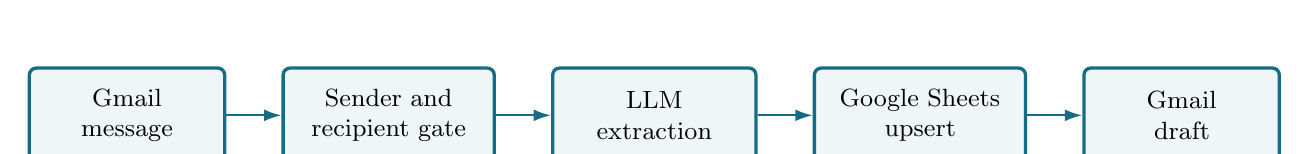
\begin{tikzpicture}[node distance=7mm]
  \node[zgstage, text width=22mm] (mail) {Gmail\\message};
  \node[zgstage, text width=24mm, right=of mail] (gate) {Sender and\\recipient gate};
  \node[zgstage, text width=23mm, right=of gate] (llm) {LLM\\extraction};
  \node[zgstage, text width=24mm, right=of llm] (sheet) {Google Sheets\\upsert};
  \node[zgstage, text width=22mm, right=of sheet] (reply) {Gmail\\draft};
  \draw[zgflow] (mail) -- (gate);
  \draw[zgflow] (gate) -- (llm);
  \draw[zgflow] (llm) -- (sheet);
  \draw[zgflow] (sheet) -- (reply);
\end{tikzpicture}
\caption{The external path exercised by the test.}
\end{figure}

ZipperGen also records where the Mailbox, Gatekeeper, Extractor, and Table
participants are in their projected programs. The deployment owns one
SQLite store and one immutable source bundle.

\section{Does running on the AI server matter?}

For ordinary Studio commands, it does not matter. Run Studio on the same
machine that will host the deployment. Paths, model settings, connector
bindings, credentials, the durable store, and the managed Python environment
then belong to that machine.

Three server details still matter:

\begin{enumerate}
  \item The server needs outbound HTTPS access to Google and to any remote
        model provider.
  \item Google authorization needs a browser callback. A server with a
        desktop browser handles this directly. An SSH-only server needs the
        small tunnel described in Section~\ref{sec:oauth}.
  \item A persistent Linux deployment needs a working user
        \texttt{systemd} manager. Some servers require an administrator to
        enable lingering for the account.
\end{enumerate}

If Ollama runs on the same AI server, use
\texttt{http://127.0.0.1:11434/v1}. No model tunnel is needed. A tunnel is
needed only when Ollama runs on a different machine.

\section{Prepare the application directory}

The outer directory is the application project. The framework checkout is a
separate nested repository:

\begin{lstlisting}[style=shell]
mkdir -p "$HOME/Projects"
cd "$HOME/Projects"
mkdir zippergen-call-intake
cd zippergen-call-intake
git init
git clone https://github.com/zippergen-io/zippergen.git zippergen
uv python install 3.12
uv sync --project zippergen --python 3.12 --extra google
\end{lstlisting}

The \texttt{google} extra is needed by the Studio process that performs OAuth
and checks Gmail and Sheets. Managed deployments detect the same connector
requirements and install this extra automatically.

Start Studio from the outer directory with the nested environment:

\begin{lstlisting}[style=shell]
cd "$HOME/Projects/zippergen-call-intake"
uv run --no-sync --project zippergen zippergen
\end{lstlisting}

The process uses the nested ZipperGen installation but keeps the outer
directory as its project root.

\section{Initialize the project and import the workflow}

At the Studio prompt, enter:

\begin{lstlisting}[style=shell]
project init call-intake-check
workflow import zippergen/examples/call_intake.py:call_intake
\end{lstlisting}

Studio copies the workflow to \path{examples/call_intake.py} in the outer
project and selects it. The nested framework repository remains separate.

Check what was imported:

\begin{lstlisting}[style=shell]
workflow files
workflow show communications
workflow show agent Mailbox
workflow show agent Extractor
workflow show full
workflow validate
\end{lstlisting}

Validation should report four participants:
\texttt{Mailbox}, \texttt{Gatekeeper}, \texttt{Extractor}, and
\texttt{Table}. It should also report the logical connector requirements
\texttt{call-mailbox} and \texttt{call-records}.

\section{Record the intended behavior}

An imported workflow is visible code, but the fresh project does not yet have
a canonical specification. Enter:

\begin{lstlisting}[style=shell]
workflow edit spec
\end{lstlisting}

Replace the initial writing guide with this text:

\begin{lstlisting}
# Call Intake

Watch a Gmail inbox for call announcements and corrections.

## Participants and behavior

- Mailbox polls Gmail and owns message completion.
- Gatekeeper accepts only configured recipients and certified senders.
- Extractor uses an LLM to classify a message as a call, correction, or other.
- Extractor converts calls and corrections into structured JSON.
- Table upserts records in Google Sheets by a stable call_id.
- Mailbox creates a reply containing the resulting JSON.
- Corrections preserve the call_id and update the existing row.
- Processing is durable and continues polling after each message.

## Safety and configuration

- Gmail and Google Sheets are logical connector requirements.
- Accounts, queries, spreadsheet IDs, tabs, and OAuth tokens stay in Studio.
- Use Gmail draft mode by default.
- Never process a sender that is not explicitly certified.
- Never process a message sent to an unexpected intake address.
- Limit automatic sending to at most ten messages per hour.
\end{lstlisting}

Save and leave the editor. Then review the recorded intent and the code:

\begin{lstlisting}[style=shell]
workflow show spec
workflow show protocol
workflow validate
workflow accept
\end{lstlisting}

\texttt{workflow accept} records the reviewed specification, semantics, and
source snapshot. It does not run or deploy anything.

\section{Configure the LLM}

The only LLM participant is \texttt{Extractor}. Use one real model so that
the extracted Sheet row is meaningful.

\subsection{Option A: Ollama on the same AI server}

\begin{lstlisting}[style=shell]
model provider configure local
model config create call-extractor
model config check call-extractor
model default call-extractor
model assignments check
\end{lstlisting}

Accept the default endpoint
\texttt{http://127.0.0.1:11434/v1}. When Studio asks for a model, enter an
identifier returned by the server, for example \texttt{qwen2.5:7b}. The
configuration check confirms the exact identifier. Studio then asks when the
model should be released after its last use. Press Enter for \texttt{300}
seconds. The call-intake workflow can continue polling Gmail without occupying
the model memory. Ollama loads the model again automatically when a new email
reaches the Extractor action. Enter \texttt{never} only when the model should
remain loaded.

\subsection{Option B: a hosted model}

For OpenAI, enter:

\begin{lstlisting}[style=shell]
model provider configure openai
model config create call-extractor
model config check call-extractor
model default call-extractor
model assignments check
\end{lstlisting}

Studio asks for the API key privately and then asks for the model name. The
same sequence works with \texttt{mistral} or \texttt{anthropic} as provider.
Configure only one option for this test.

\section{Prepare Google}

Use one Google account for Gmail and the test Sheet.

\begin{enumerate}
  \item Create or select a Google Cloud project.
  \item Enable the Gmail API.
  \item Enable the Google Sheets API.
  \item Configure the OAuth consent screen.
  \item If the application is in external testing mode, add the Gmail account
        as a test user.
  \item Create an OAuth client of type \emph{Desktop app}.
  \item Download the client JSON file.
  \item Create an empty spreadsheet and name one tab \texttt{Calls}.
\end{enumerate}

Keep the downloaded JSON outside the application repository. Do not create a
server directory, choose a permanent server filename, or change permissions
yourself. Studio imports the client into its private storage.

\section{Configure Gmail and Sheets in Studio}
\label{sec:oauth}

Return to the Studio prompt and enter:

\begin{lstlisting}[style=shell]
connector setup
\end{lstlisting}

Studio asks for:

\begin{enumerate}
  \item whether the OAuth desktop client JSON is already on the AI server or
        must be uploaded
  \item Google authorization in a browser
  \item a Gmail search query
  \item a spreadsheet URL or ID
  \item the tab name
\end{enumerate}

If the JSON is already on the AI server, select
\emph{Use a file already on this computer} and enter its path. Studio validates
and imports it, so the original file is not needed afterward.

If the JSON is on your local computer, select
\emph{Upload from another computer}. Enter its absolute local path and the SSH
host or alias used for the AI server. Studio creates a private temporary
destination and prints one complete \texttt{scp} command. Run that single
command in a local terminal, then return to Studio and press Enter. Studio
validates and imports the client and removes the temporary upload. Later
authorization changes reuse the privately stored client, so no path is asked
for again.

A useful test query is:

\begin{lstlisting}
is:unread in:inbox to:call-intake+test@example.com
\end{lstlisting}

Replace the address with the real test recipient. Later, enter the spreadsheet
URL and tab \texttt{Calls}.

\begin{notebox}{OAuth on an SSH-only server}
Studio detects an interactive SSH session and chooses an available callback
port before authorization starts. It prints exact commands for a multiplexed
SSH connection. In a second terminal on the local computer, first check the
master connection and then add the displayed forwarding rule:
\begin{lstlisting}[style=shell]
ssh -O check AI_SERVER
ssh -O forward -L 48321:127.0.0.1:48321 AI_SERVER
\end{lstlisting}
If no SSH master is configured, Studio also displays the equivalent
\texttt{ssh -N -L} command, which must remain open in its terminal. Return to
Studio and press Enter. Copy the Google authorization URL that appears into
the local browser. After Google redirects the browser to
\texttt{localhost:48321}, the tunnel carries the callback to Studio. Studio
prints the cleanup command after authorization. Use the actual port displayed
by Studio, not \texttt{48321}.
\end{notebox}

Studio requests Gmail and Sheets scopes because this workflow reads and
modifies both services. It stores the resulting refresh credential privately.
The project files contain no token.

Check the complete connector state:

\begin{lstlisting}[style=shell]
connector
connector provider check google
connector assignments check
\end{lstlisting}

The expected bindings are:

\begin{center}
\begin{tabularx}{0.94\linewidth}{@{}l l l X@{}}
\toprule
Requirement & Participant & Kind & Configuration contains \\
\midrule
\texttt{call-mailbox} & Mailbox & Gmail & account and search query \\
\texttt{call-records} & Table & Sheets & spreadsheet ID and tab \\
\bottomrule
\end{tabularx}
\end{center}

\section{Prepare the deployment without starting it}

Enter:

\begin{lstlisting}[style=shell]
deploy call-intake-check --no-start
\end{lstlisting}

Choose these safe values when Studio asks:

\begin{center}
\begin{tabularx}{0.94\linewidth}{@{}l X@{}}
\toprule
Question & Test value \\
\midrule
External services & \texttt{live} \\
Certified senders & one exact address that you control \\
Intake recipient & the address used in the Gmail query \\
Reply mode & \texttt{draft} \\
Maximum replies per hour & \texttt{2} \\
Polling interval & \texttt{15} seconds \\
\bottomrule
\end{tabularx}
\end{center}

Studio creates the immutable bundle, managed Python environment, private
deployment secrets, profile, log path, and empty durable store. It does not
start the service because of \texttt{--no-start}.

Inspect readiness:

\begin{lstlisting}[style=shell]
deploy show call-intake-check
deploy doctor call-intake-check
deploy inspect call-intake-check
\end{lstlisting}

The store should already exist. The run may say that durable execution has not
started yet. That is expected.

\section{Send one controlled test message}

Send an email that satisfies both configured gates:

\begin{itemize}
  \item \textbf{From}: the exact certified sender
  \item \textbf{To}: the exact intake recipient
  \item \textbf{Subject}: \texttt{Test call for formal methods projects}
\end{itemize}

Example body:

\begin{lstlisting}
The Example Research Fund has opened a call for formal-methods projects.
Applications close on 2026-10-15.
Funding is up to EUR 100,000 for 24 months.
More information: https://example.org/formal-methods-call
\end{lstlisting}

Leave the message unread until the deployment starts.

\section{Start and observe the service}

In Studio, enter:

\begin{lstlisting}[style=shell]
deploy start call-intake-check
deploy show call-intake-check
deploy logs call-intake-check
\end{lstlisting}

Repeat \texttt{deploy logs call-intake-check} when you want the newest log
output. Reading the log does not stop the managed deployment.

In another Studio terminal opened from the same outer project directory, use:

\begin{lstlisting}[style=shell]
deploy inspect call-intake-check
deploy trace call-intake-check
\end{lstlisting}

The inspection view shows the latest durable local-program position for each
participant. During normal polling, Mailbox may be waiting in
\texttt{wait\_briefly}. While the model is active, Extractor may be at an LLM
action. Table appears at the Sheets effect while a row is written.

\section{Check the external result}

The first successful message should produce all of the following:

\begin{enumerate}
  \item The original Gmail message is no longer unread.
  \item The \texttt{Calls} tab contains a header and one row.
  \item The row contains a stable \texttt{call\_id}.
  \item Gmail Drafts contains a reply with the extracted JSON.
  \item \texttt{deploy show call-intake-check} reports a running service and
        an existing store.
  \item \texttt{deploy trace call-intake-check} shows the participant events.
\end{enumerate}

If the Sheet row exists but no draft appears, inspect:

\begin{lstlisting}[style=shell]
deploy logs call-intake-check
deploy doctor call-intake-check
\end{lstlisting}

If nothing happens, first confirm that the message is unread and matches the
configured Gmail query. Then confirm the exact sender and recipient values.

\section{Stop or remove the deployment}

Stop the service after the test:

\begin{lstlisting}[style=shell]
deploy stop call-intake-check
deploy show call-intake-check
\end{lstlisting}

Stopping preserves the profile, immutable bundle, log, and durable store. It
can be started again with:

\begin{lstlisting}[style=shell]
deploy start call-intake-check
\end{lstlisting}

To remove the service registration but keep recoverable deployment data, use:

\begin{lstlisting}[style=shell]
deploy remove call-intake-check
\end{lstlisting}

Use the purge option only when the test data is no longer needed:

\begin{lstlisting}[style=shell]
deploy remove call-intake-check --purge
\end{lstlisting}

Studio asks for the deployment name and confirmation before permanent
deployment data is removed. The Google spreadsheet, Gmail messages, drafts,
and Google Cloud OAuth client are external resources. Purging a ZipperGen
deployment does not delete them.

\section{Keeping it alive after SSH logout}

On Linux, Studio uses a user \texttt{systemd} service when it is available.
Check it through Studio:

\begin{lstlisting}[style=shell]
deploy show call-intake-check
deploy doctor call-intake-check
\end{lstlisting}

If the service stops when the final SSH session closes, ask the server
administrator whether lingering is enabled for your account. The usual
administrator command is:

\begin{lstlisting}[style=shell]
loginctl enable-linger USERNAME
\end{lstlisting}

This is account-level server policy, so Studio does not change it
automatically. It is not needed for a short test while the SSH session remains
open.

\section{Compact command sheet}

\begin{lstlisting}[style=shell]
# Run from the outer project directory
uv run --no-sync --project zippergen zippergen

# Studio commands
project init call-intake-check
workflow import zippergen/examples/call_intake.py:call_intake
workflow edit spec
workflow show communications
workflow show full
workflow validate
workflow accept

model provider configure local
model config create call-extractor
model config show call-extractor
model default call-extractor
model assignments check

connector setup
connector assignments check

deploy call-intake-check --no-start
deploy doctor call-intake-check
deploy start call-intake-check
deploy show call-intake-check
deploy inspect call-intake-check
deploy trace call-intake-check
deploy logs call-intake-check
deploy stop call-intake-check
\end{lstlisting}

\begin{notebox}{Success criterion}
The end-to-end check is complete when one controlled unread email becomes one
Google Sheets row and one Gmail draft, while Studio reports a running
deployment with an existing durable store.
\end{notebox}

\end{document}
